\chapter*{Spremanje izmjena}
\addcontentsline{toc}{chapter}{Spremanje izmjena}

Vratimo se na trenutak na naša dva primjera, linerani model verzioniranja koda:

\input{graphs/linearni_model}

\dots{}i primjer s granama:

\input{graphs/primjer_s_granama_i_spajanjima}

U oba slučaja, čvorovi tih grafova su stanje projekta u nekom trenutku.
Na primjer, kad ste prvi put inicirali projekt s \verb+git init+, dodali ste nekoliko datoteka i \emph{spremili ih}. 
U tom trenutku je nastao čvor \emph a.
Nakon toga ste možda izmijenili neke od tih datoteka, možda neke obrisali, neke nove dodali i opet -- spremili novo stanje i dobili stanje \emph b.

To što ste radili između svaka dva stanja je vaša stvar i ne tiče se gita.
No, trenutak kad se odlučite spremiti novo stanje projekta u vaš repozitorij -- to je gitu jedino važno i to se zove \emph{commit}.

Važno je ovdje napomenuti da u gitu, za razliku od subversiona, CVS-a ili TFS-a \emph{nikad ne commitate u udaljeni repozitorij}. 
Svoje lokalne promjene \emph{commit}ate, odnosno \emph{spremate} u \emph{lokalni} repozitorij.
Interakcija s udaljenim repozitorijem će biti tema poglavlja o udaljenim repozitorijima\ref{udaljeni_repozitoriji}.

\section*{Status}
\addcontentsline{toc}{section}{Status}

Da biste provjerili imate li uopće nešto za spremati, koristi se naredba \verb+git status+.
Na primjer, kad na projektu koji nema lokalnih izmjena za spremanje utipkate \verb+git status+, dobiti ćete:

\input{git_output/git_status_0}

Pretpostavimo da ste odlučili napraviti tri izmjene na projektu. i
Izmijenili ste liniju u datoteci \verb+README.md+ i \verb+setup.py+ i obrisali \verb+TODO.txt+:
Sad će rezultat od \verb+git status+ izgledati ovako:

\input{git_output/git_status_1}

Najbitniji podatak je linija u kojoj piše \verb+modified: git-commit.tex+, jer to je datoteka koju sam \emph{mijenjao}, ali ne još snimio.

Želite li pogledati \emph{koje su točne razlike} u tim datotekama u odnosu na stanje kakvo je snimljeno u repozitoriju, odnosno u \emph{zadnjoj verziji} repozitorija, to ćete dobiti s \verb+git diff+. 
Opet, u slučaju moje knjige, taj ispis izgleda ovako nekako:

\input{git_output/git_diff_1}

Ako vam ovo izgleda zbunjujuće -- postoji i način kako da se to ljepše prikaže, no, čisto za vježbu, nije loše pokušati interpretirati što ovo znači.
Najvažniji dijelovi su linije oni koji počinju si \verb+diff+, jer one govore o kojim datotekama se radi.
Nakon njih slijedi nekoliko linija s općenitim podacima i zatim kod \emph{oko} dijela koji je izmijenjen i onda ono najvažnije -- linije obojane u crveno i one obojane u plavo.

Linije koje započinju s "-" (crvene) su linije koje su \emph{obrisane}, a one koje počinju s "+" (u plavom) su one koje su \emph{dodane}. 
Primijetite da git ne zna da ste neku liniju izmijenili. 
Ukoliko jeste -- on se ponaša kao da ste staru obrisalu, a novu dodali.

Rezultat git naredbe su samo dijelovi koje ste izmijenili i nekoliko linija \emph{oko njih}.
Ukoliko želite malo veću tu "okolinu" oko vaših izmjena, možete ju izmijeniti s opcijom \verb+-U<broj_linija>+.
Na primjer, ukoliko želite 10 linija oko izmjenjenih dijelova koda, to ćete dobiti sa:

\gitoutputcommand{git diff -U10}

\section*{Međuprostor za commit}
\addcontentsline{toc}{section}{Međuprostor za commit}

U gitu postoji poseban "prostor" u koje se "stavljaju" datoteke koje ćete spremiti (\emph{commit}ati):

\input{git_output/git_add_1}

Ili jednostavnije:

\input{git_output/git_add_2}

Nakon toga, rezultat od \verb+git status+ je:

\input{git_output/git_status_2}

Ukoliko ima neka datoteka koju ste staviti u međuprostor za \emph{commit}, ali ste se kasnije predomislili. 
Sad tu datoteku želite izbaciti, ali bez da gubite izmjene koje ste na njemu napravili jer će one biti dio nekog sljedećeg \emph{commit}a.
To se može naredbom:

\gitoutputcommand{git rm --cached <datoteka1> <datoteka2> \dots}

Događati će vam se da ste promijenili neku datoteku, no kasnije se ispostavilo da ta izmjena nije bila potrebna. 
I sad ju ne želite spremiti nego vratiti u prethodno stanje.
To se može ovako:

\gitoutputcommand{git checkout HEAD -- <datoteka1> <datoteka2> \dots}

Više detalja o \verb+git checkout+ i zašto ova gornja naredba radi to što radi biti će u poglavlju o granama grananju.

\section*{Prvi commit}
\addcontentsline{toc}{section}{Prvi commit}

Izmjene možete spremiti s:

\gitoutputcommand{git commit -m "Nova verzija"}

U stringu nakon \verb+-m+ \emph{morate} unijeti komentar uz svaku promjenu koju spremate na projektu.
Git ne dopušta spremanje izmjena bez komentara.

Sad je status projekta opet:

\input{git_output/git_status_0}

\dots{}a sve prethodne izmjene možete pogledati s \verb+git log+:

\input{git_output/git_log_0}

\section*{Ispravljanje zadnje izmjene}
\addcontentsline{toc}{section}{Ispravljanje zadnje izmjene}

Dogoditi će vam se da spremite neku izmjenu u repozitorij, gledate još malo projekt i shvatite da ste mogli još jednu sitnicu napraviti.
I, nekako vam se čini da bi bilo logično da ta sitnica bude dio prethodnog \emph{commit}a.

Bilo bi lijepo, pomislit' ćete kad biste mogli izmijeniti zadnji \emph{commit} tako da sadrži i ovu novu, sitnu, ispravku koju ste dodali.
S gitom se to može.
Prvo \emph{napravite} tu izmjenu; recimo da je ona bila na datotecu \verb+README.md+, dodate tu datoteku u naš međuprostor za izmjene s \verb+git add README.md+ i izvršite sljedeće:

\gitoutputcommand{git commit --amend -m "Nova verzija, promijenjen README.md"}

Ukoliko provjerite s \verb+git log+ šte se desilo, otkriti ćete da zadnji \emph{commit} sad ima novi komentar.
U stvari, ispravno bi bilo kazati da je promijenjen i cijeli taj \emph{commit}.

\section*{Git gui}
\addcontentsline{toc}{section}{Git gui}

Kad spremate neku izmjenu koja ima puno datoteka, onda je gnjavaža non stop tipkati \verb+git add+.
Zbog toga postoji poseban grafički program kojemu je glavna namjena upravo to.
Kad u komandnoj liniji utipkate:

\gitoutputcommand{git gui}

Otvoriti će se sljedeće:

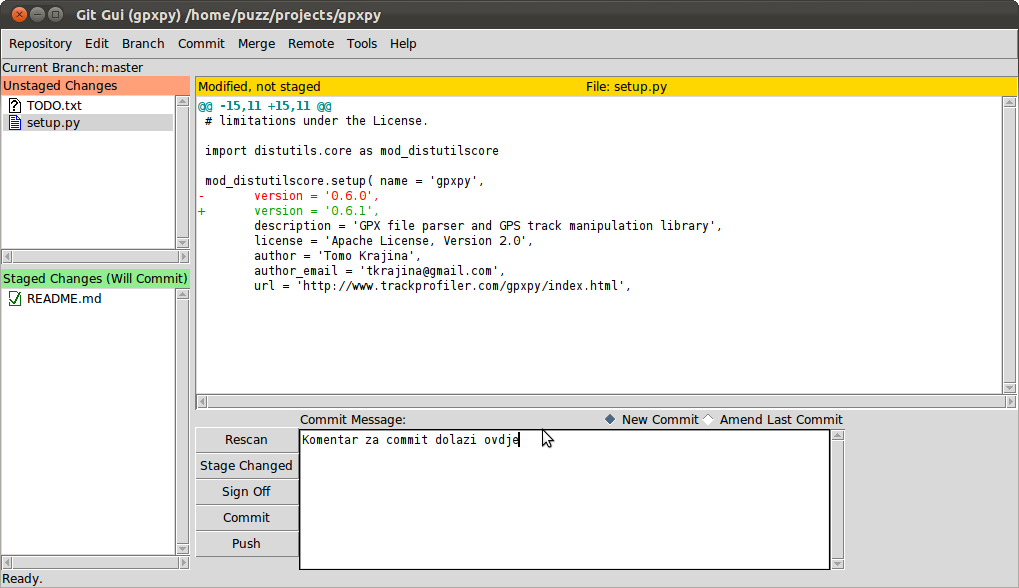
\includegraphics[width=14cm]{images/git-gui.png}

Program se sastoji od četiri polja. 

\begin{itemize}
	\item Polje za datoteke koje su izmijenjene, ali nisu još u međuprostoru za snimanje izmjena (gore lijevo).
	\item Polje za prikaz izmjena u pojedinim datotekama (gore desno). 
	\item Polje za datoteke koje su izmijenjene i stavljene su u međuprostor za \emph{commit} (dolje lijevo).
	\item Polje za \emph{commit} (dolje lijevo).
\end{itemize}

Kad kliknete na neku datoteku, prikazati će se sve izmjene koja ta datoteka sadrži u odnosu na zadnje snimljeno stanje u repozitoriju.
Format je isti kao i kod \verb+git diff+.
Klik na ikonu uz naziv datoteke će istu prebaciti iz polja izmijenjenih datotke u polje izmijenjenih i spremnih za \emph{commit} i suprotno.
Upišite komentar i kliknite na \emph{Commit} za snimanje izmjene.

Ovdje, kao i u radu s komandnom linijom ne morati sve izmijenjene datoteke snimiti u jednom \emph{commit}u. 
Možete dodati nekoliko datoteka, upisati komentar, snimiti i nakon toga dodati sljedećih nekoliko datoteka, opisati novi komentar i snimiti sljedeću izmjenu.
Koristite li \verb+git gui+ onda ovdje imati još jednu korisnu opciju, možete u međuprostor za commit dodati ne \emph{cijelu} datoteku, nego samo \emph{nekoliko izmijenjenih linija}.
Odaberite datoteku, u polju s izmijenjenim linijama odaberite samo linije koje želite spremite, desni klik i:

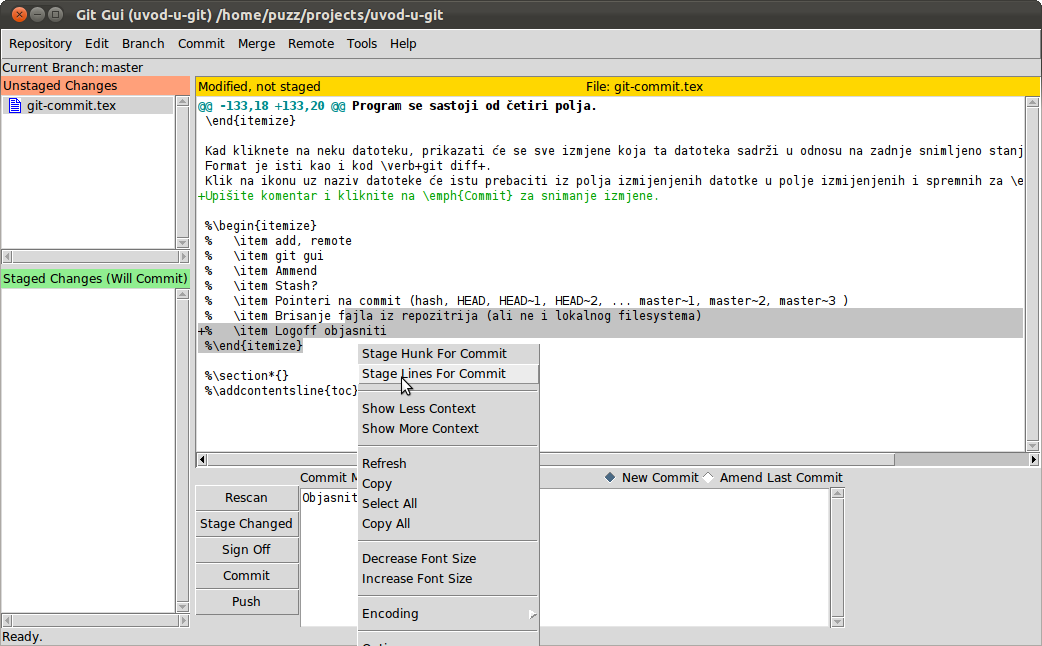
\includegraphics[width=14cm]{images/git-gui-stage-lines-to-commit.png}

Više puta će vam se dogoditi da ste na nekoj datoteci napravili izmjenu koju \emph{ne} želite snimiti. 
Takvu datoteku možete resetirati, odnosno vratiti u početno stanje tako da ju odaberete u meniju \verb+Commit+ $\rightarrow$ \verb+Revert changes+.

Osim ovoga, \verb+git gui+ ima puno korisnih mogućnosti koje nisu predmet ovog poglavlja.
Preporučam van da nađete vremena i proučite sve menije i kratice s tastaturom u radu s \verb+git gui+ jer to će vam drastično ubrzati rad s ovim korisnim programčićem.

%\begin{itemize}
%   \item Tipični scenarij
%   \item Stash?
%   \item Pointeri na commit (hash, HEAD, HEAD~1, HEAD~2, ... master~1, master~2, master~3 )
%   \item Brisanje fajla iz repozitrija (ali ne i lokalnog filesystema)
%   \item Logoff objasniti
%\end{itemize}

%\section*{}
%\addcontentsline{toc}{section}{}

